\begin{exercice}
    Que peut-on dire sur une fonction concave et positive sur $\R$ ?
\end{exercice}

\begin{elem_sol}
    Faire un dessin...
\end{elem_sol}


\begin{marginfigure}[-4cm]
\centering
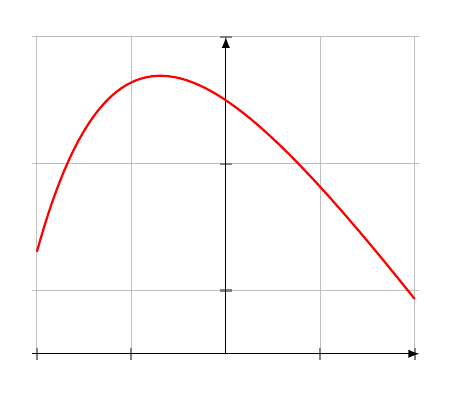
\begin{tikzpicture}
    \begin{axis}[width=6.5cm,
        axis lines=middle,
        axis line style={-latex},
        grid=major,
        xmin=-4.1, xmax=4.1,
        ymin=5, ymax=10,
        xticklabels=\empty,
        yticklabels=\empty,
        tick style={thick},
        ticklabel style={font=\normalsize},
    ]
    \def\a{-4}
    \def\b{4}
    \addplot[red,thick,samples=100,domain=\a:\b] {-(x+exp(-x/2)) + 10};
    \end{axis}
\end{tikzpicture}
\end{marginfigure}